\documentclass[a4paper,12pt,twoside]{memoir}

% Castellano
\usepackage[spanish,es-tabla]{babel}
\selectlanguage{spanish}
\usepackage[utf8]{inputenc}
\usepackage[T1]{fontenc}
\usepackage{lmodern} % Scalable font
\usepackage{microtype}
\usepackage{placeins}
\usepackage{float}

\RequirePackage{booktabs}
\RequirePackage[table]{xcolor}
\RequirePackage{xtab}
\RequirePackage{multirow}

\usepackage{pdfpages}

% Links
\usepackage[colorlinks]{hyperref}
\hypersetup{
	allcolors = {red}
}

% Ecuaciones
\usepackage{amsmath}
\usepackage{amssymb}

\newcommand{\hubu}{\hline \rule{0pt}{2.7ex}}
\usepackage{eurosym} % para el euro

% Rutas de fichero / paquete
\newcommand{\ruta}[1]{{\sffamily #1}}

% Párrafos
\nonzeroparskip


\clubpenalty=10000
\widowpenalty=10000
% Evitar solapes en el header
\nouppercaseheads

\usepackage[ruled,vlined]{algorithm2e}

\usepackage{pdflscape}

% Imagenes
\usepackage{graphicx}
\newcommand{\imagen}[2]{
	\begin{figure}[!h]
		\centering
		\includegraphics[width=0.9\textwidth]{#1}
		\caption{#2}\label{fig:#1}
	\end{figure}
	\FloatBarrier
}

\newcommand{\imagenflotante}[2]{
	\begin{figure}%[!h]
		\centering
		\includegraphics[width=0.9\textwidth]{#1}
		\caption{#2}\label{fig:#1}
	\end{figure}
}



% El comando \figura nos permite insertar figuras comodamente, y utilizando
% siempre el mismo formato. Los parametros son:
% 1 -> Porcentaje del ancho de página que ocupará la figura (de 0 a 1)
% 2 --> Fichero de la imagen
% 3 --> Texto a pie de imagen
% 4 --> Etiqueta (label) para referencias
% 5 --> Opciones que queramos pasarle al \includegraphics
% 6 --> Opciones de posicionamiento a pasarle a \begin{figure}
\newcommand{\figuraConPosicion}[6]{%
  \setlength{\anchoFloat}{#1\textwidth}%
  \addtolength{\anchoFloat}{-4\fboxsep}%
  \setlength{\anchoFigura}{\anchoFloat}%
  \begin{figure}[#6]
    \begin{center}%
      \Ovalbox{%
        \begin{minipage}{\anchoFloat}%
          \begin{center}%
            \includegraphics[width=\anchoFigura,#5]{#2}%
            \caption{#3}%
            \label{#4}%
          \end{center}%
        \end{minipage}
      }%
    \end{center}%
  \end{figure}%
}

%
% Comando para incluir imágenes en formato apaisado (sin marco).
\newcommand{\figuraApaisadaSinMarco}[5]{%
  \begin{figure}%
    \begin{center}%
    \includegraphics[angle=90,height=#1\textheight,#5]{#2}%
    \caption{#3}%
    \label{#4}%
    \end{center}%
  \end{figure}%
}
% Para las tablas
\newcommand{\otoprule}{\midrule [\heavyrulewidth]}
%
% Nuevo comando para tablas pequeñas (menos de una página).
\newcommand{\tablaSmall}[5]{%
 \begin{table}
  \begin{center}
   \rowcolors {2}{gray!35}{}
   \begin{tabular}{#2}
    \toprule
    #4
    \otoprule
    #5
    \bottomrule
   \end{tabular}
   \caption{#1}
   \label{tabla:#3}
  \end{center}
 \end{table}
}

%
% Nuevo comando para tablas pequeñas (menos de una página).
\newcommand{\tablaSmallSinColores}[5]{%
 \begin{table}[H]
  \begin{center}
   \begin{tabular}{#2}
    \toprule
    #4
    \otoprule
    #5
    \bottomrule
   \end{tabular}
   \caption{#1}
   \label{tabla:#3}
  \end{center}
 \end{table}
}

\newcommand{\tablaApaisadaSmall}[5]{%
\begin{landscape}
  \begin{table}
   \begin{center}
    \rowcolors {2}{gray!35}{}
    \begin{tabular}{#2}
     \toprule
     #4
     \otoprule
     #5
     \bottomrule
    \end{tabular}
    \caption{#1}
    \label{tabla:#3}
   \end{center}
  \end{table}
\end{landscape}
}

%
% Nuevo comando para tablas grandes con cabecera y filas alternas coloreadas en gris.
\newcommand{\tabla}[6]{%
  \begin{center}
    \tablefirsthead{
      \toprule
      #5
      \otoprule
    }
    \tablehead{
      \multicolumn{#3}{l}{\small\sl continúa desde la página anterior}\\
      \toprule
      #5
      \otoprule
    }
    \tabletail{
      \hline
      \multicolumn{#3}{r}{\small\sl continúa en la página siguiente}\\
    }
    \tablelasttail{
      \hline
    }
    \bottomcaption{#1}
    \rowcolors {2}{gray!35}{}
    \begin{xtabular}{#2}
      #6
      \bottomrule
    \end{xtabular}
    \label{tabla:#4}
  \end{center}
}

%
% Nuevo comando para tablas grandes con cabecera.
\newcommand{\tablaSinColores}[6]{%
  \begin{center}
    \tablefirsthead{
      \toprule
      #5
      \otoprule
    }
    \tablehead{
      \multicolumn{#3}{l}{\small\sl continúa desde la página anterior}\\
      \toprule
      #5
      \otoprule
    }
    \tabletail{
      \hline
      \multicolumn{#3}{r}{\small\sl continúa en la página siguiente}\\
    }
    \tablelasttail{
      \hline
    }
    \bottomcaption{#1}
    \begin{xtabular}{#2}
      #6
      \bottomrule
    \end{xtabular}
    \label{tabla:#4}
  \end{center}
}

%
% Nuevo comando para tablas grandes sin cabecera.
\newcommand{\tablaSinCabecera}[5]{%
  \begin{center}
    \tablefirsthead{
      \toprule
    }
    \tablehead{
      \multicolumn{#3}{l}{\small\sl continúa desde la página anterior}\\
      \hline
    }
    \tabletail{
      \hline
      \multicolumn{#3}{r}{\small\sl continúa en la página siguiente}\\
    }
    \tablelasttail{
      \hline
    }
    \bottomcaption{#1}
  \begin{xtabular}{#2}
    #5
   \bottomrule
  \end{xtabular}
  \label{tabla:#4}
  \end{center}
}



\definecolor{cgoLight}{HTML}{EEEEEE}
\definecolor{cgoExtralight}{HTML}{FFFFFF}

%
% Nuevo comando para tablas grandes sin cabecera.
\newcommand{\tablaSinCabeceraConBandas}[5]{%
  \begin{center}
    \tablefirsthead{
      \toprule
    }
    \tablehead{
      \multicolumn{#3}{l}{\small\sl continúa desde la página anterior}\\
      \hline
    }
    \tabletail{
      \hline
      \multicolumn{#3}{r}{\small\sl continúa en la página siguiente}\\
    }
    \tablelasttail{
      \hline
    }
    \bottomcaption{#1}
    \rowcolors[]{1}{cgoExtralight}{cgoLight}

  \begin{xtabular}{#2}
    #5
   \bottomrule
  \end{xtabular}
  \label{tabla:#4}
  \end{center}
}


\graphicspath{ {./img/} }

% Capítulos
\chapterstyle{bianchi}
\newcommand{\capitulo}[2]{
	\setcounter{chapter}{#1}
	\setcounter{section}{0}
	\chapter*{#2}
	\addcontentsline{toc}{chapter}{#1. #2}
	\markboth{#2}{#2}
}

% Apéndices
\renewcommand{\appendixname}{Apéndice}
\renewcommand*\cftappendixname{\appendixname}

\newcommand{\apendice}[1]{
	%\renewcommand{\thechapter}{A}
	\chapter{#1}
}

\renewcommand*\cftappendixname{\appendixname\ }

% Formato de portada
\makeatletter
\usepackage{xcolor}
\newcommand{\tutor}[1]{\def\@tutor{#1}}
\newcommand{\course}[1]{\def\@course{#1}}
\definecolor{cpardoBox}{HTML}{E6E6FF}
\def\maketitle{
  \null
  \thispagestyle{empty}
  % Cabecera ----------------
\begin{center}%
	{\noindent\Huge Universidades de Burgos, León y Valladolid}\vspace{.5cm}%
	
	{\noindent\Large Máster universitario}\vspace{.5cm}%
	
	{\noindent\Huge \textbf{Inteligencia de Negocio y Big~Data en Entornos Seguros}}\vspace{.5cm}%
\end{center}%

\begin{center}%
	
\includegraphics[height=3cm]{img/escudoUBU} \hspace{1cm}
	
\includegraphics[height=3cm]{img/escudoUVA} \hspace{1cm}
	
\includegraphics[height=3cm]{img/escudoULE} \vspace{1cm}%
\end{center}%

  \vfill
  % Título proyecto y escudo informática ----------------
  \colorbox{cpardoBox}{%
    \begin{minipage}{.9\textwidth}
      \vspace{.2cm}\Large
      \begin{center}
      \textbf{Trabajo Fin de Máster}\vspace{.6cm}\\
      \textbf{\LARGE\@title{}}
      \end{center}
      \vspace{.2cm}
    \end{minipage}

  }%
  
  \vfill
  % Datos de alumno, curso y tutores ------------------
  \begin{center}%
  {%
    \noindent\LARGE
    Presentado por \@author{}\\ 
    en Universidad de Burgos --- \@date{}\\
    Tutores: \@tutor{}\\
  }%
  \end{center}%
  \null
  \cleardoublepage
  }
\makeatother

\usepackage{subcaption}


% Default fixed font does not support bold face
\DeclareFixedFont{\ttb}{T1}{txtt}{bx}{n}{12} % for bold
\DeclareFixedFont{\ttm}{T1}{txtt}{m}{n}{12}  % for normal

% Custom colors
\usepackage{color}
\definecolor{deepblue}{rgb}{0,0,0.5}
\definecolor{deepred}{rgb}{0.6,0,0}
\definecolor{deepgreen}{rgb}{0,0.5,0}

\usepackage{listings}

% Python style for highlighting
\newcommand\pythonstyle{\lstset{
		language=Python,
		basicstyle=\ttm,
		otherkeywords={self},             % Add keywords here
		keywordstyle=\ttb\color{deepblue},
		emph={MyClass,__init__},          % Custom highlighting
		emphstyle=\ttb\color{deepred},    % Custom highlighting style
		stringstyle=\color{deepgreen},
		frame=tb,                         % Any extra options here
		showstringspaces=false            % 
}}
% Python environment
\lstnewenvironment{python}[1][]
{
	\pythonstyle
	\lstset{#1}
}
{}

% Python for external files
\newcommand\pythonexternal[2][]{{
		\pythonstyle
		\lstinputlisting[#1]{#2}}}

% Python for inline
\newcommand\pythoninline[1]{{\pythonstyle\lstinline!#1!}}

\usepackage{dirtree}


\newcommand{\nombre}{Willow Maui García Moreno} %%% cambio de comando

% Datos de portada
\title{Desarrollo de un prototipo de delimitación automática de parcelas a partir de imágenes de satélite}
\author{\nombre}
\tutor{Dr. José Francisco Díez Pastor}
\date{\today}

\begin{document}

\maketitle


\newpage\null\thispagestyle{empty}\newpage


%%%%%%%%%%%%%%%%%%%%%%%%%%%%%%%%%%%%%%%%%%%%%%%%%%%%%%%%%%%%%%%%%%%%%%%%%%%%%%%%%%%%%%%%
\thispagestyle{empty}


\noindent
\begin{center}%
	{\noindent\Huge Universidades de Burgos, León y Valladolid}\vspace{.5cm}%
	
\begin{center}%
	
\includegraphics[height=3cm]{img/escudoUBU} \hspace{1cm}
	
\includegraphics[height=3cm]{img/escudoUVA} \hspace{1cm}
	
\includegraphics[height=3cm]{img/escudoULE} \vspace{1cm}%
\end{center}%

	{\noindent\Large \textbf{Máster universitario en Inteligencia de Negocio y Big~Data en Entornos Seguros}}\vspace{.5cm}%
\end{center}%



\noindent D. José Francisco Díez Pastor, profesor del departamento de Ingeniería Informática, área de Lenguajes y Sistemas Informáticos.

\noindent Expone:

\noindent Que el alumno D. \nombre, con DNI 71706742X, ha realizado el Trabajo final de Máster en Inteligencia de Negocio y Big Data en Entornos Seguros 
          titulado Desarrollo de un prototipo de delimitación automática de parcelas a partir de imágenes de satélite. 

\noindent Y que dicho trabajo ha sido realizado por el alumno bajo la dirección del que suscribe, en virtud de lo cual se autoriza su presentación y defensa.

\begin{center} %\large
En Burgos, {\large \today}
\end{center}

\vfill\vfill\vfill

% Author and supervisor
%\begin{minipage}{0.45\textwidth}
%\begin{flushleft} %\large
%Vº. Bº. del Tutor:\\[2cm]
%Dr. José Francisco Díez Pastor
%\end{flushleft}
%\end{minipage}
%\hfill
%\begin{minipage}{0.45\textwidth}
%\begin{flushleft} %\large
%Vº. Bº. del co-tutor:\\[2cm
%
%\end{flushleft}
%\end{minipage}
%\hfill

%\vfill

% para casos con solo un tutor comentar lo anterior
% y descomentar lo siguiente
Vº. Bº. del Tutor:\\[2cm]
Dr. José Francisco Díez Pastor

\newpage\null\thispagestyle{empty}\newpage




\frontmatter

% Abstract en castellano
\renewcommand*\abstractname{Resumen}
\begin{abstract} 
	En el contexto de la agricultura, la detección precisa de los límites de las parcelas agrícolas es fundamental para una amplia gama de aplicaciones, como la gestión eficiente de los cultivos, el monitoreo de la producción y los rendimientos, el cumplimiento normativo y la solicitud de subvenciones, el análisis de cambios en el uso del suelo, y la gestión de la propiedad de la tierra.
	
	En este trabajo, los autores del artículo ``AI4Boundaries: an open AI-ready dataset to map field boundaries with Sentinel-2 and aerial photography'' presentan un dataset compuesto por imágenes satelitales del satélite Sentinel-2 y ortofotos de varios países europeos, con el objetivo de abordar el reto de la detección automática de los límites de las parcelas. Utilizando este conjunto de datos, se entrenaron diversos modelos de inteligencia artificial, con especial énfasis en una red neuronal convolucional de tipo U-Net, para evaluar su eficacia en la tarea de delimitación de los campos de cultivo.
	
	Los resultados obtenidos en este estudio sientan las bases para futuras investigaciones en este campo de gran relevancia para el sector agrícola, al demostrar el potencial de las técnicas de aprendizaje automático para automatizar la detección de los límites de las parcelas a partir de imágenes satelitales y aéreas.
\end{abstract}

\renewcommand*\abstractname{Descriptores}
\begin{abstract}
Visión artificial, \textit{Big Data}, Machine Learning, Redes neuronales convolucionales, Inteligencia artificial, Detección de bordes.
\end{abstract}

\clearpage

% Abstract en inglés
\renewcommand*\abstractname{Abstract}
\begin{abstract}
In the context of agriculture, the precise detection of agricultural field boundaries is crucial for a wide range of applications, such as efficient crop management, production and yield monitoring, regulatory compliance and subsidy application, analysis of land use changes, and land property management.

In this work, the authors of the article ``AI4Boundaries: an open AI-ready dataset to map field boundaries with Sentinel-2 and aerial photography'' present a dataset composed of Sentinel-2 satellite images and orthophotos from several European countries, with the aim of addressing the challenge of automatic detection of field boundaries. Using this dataset, various AI models were trained, with a particular emphasis on a U-Net convolutional neural network, to evaluate their effectiveness in the task of delineating croplands.

The results obtained in this study lay the groundwork for future research in this highly relevant field for the agricultural sector, by demonstrating the potential of machine learning techniques to automate the detection of field boundaries from satellite and aerial imagery.

\end{abstract}

\renewcommand*\abstractname{Keywords}
\begin{abstract}
Computer vision, \textit{Big Data}, Machine Learning,Convolutional neural networks, Artifical Intelligences, border detection.
\end{abstract}

\clearpage

% Indices
\tableofcontents

\clearpage

\listoffigures

\clearpage

\listoftables
\clearpage

\mainmatter

\addcontentsline{toc}{part}{Memoria}
\part*{Memoria}

\chapter{Introducción}

En la actualidad, en el contexto de la agricultura, los límites de las parcelas son un aspecto muy relevante, ya que nos permiten conocer la extensión de cada tipo de cultivo y su ubicación. Además, estos límites son fundamentales para cuestiones relacionadas con la propiedad de los terrenos y los posibles impuestos asociados.

El problema radica en que estos límites son cambiantes por diversos motivos, como pueden ser los cambios de propiedad o la unión de varios campos de cultivo el mismo tipo. Si bien existen registros de la propiedad que dividen estas parcelas en muchos países, estos no siempre representan la realidad de las mismas, no las cubren en su totalidad a lo largo del mundo y pueden ser complejos de consultar y analizar de forma automática.

Para abordar este problema, los autores del artículo \textit{``AI4Boundaries: an open AI-ready dataset to map field boundaries with Sentinel-2 and aerial photography''} \cite{AI4boundaries} recopilaron una serie de imágenes satelitales, las clasificaron y realizaron una separación de los terrenos en base a las bases de datos regionales de cada uno de los países involucrados. Estas imágenes proceden de Austria, España (concretamente de Cataluña), Francia, Luxemburgo, Países Bajos, Eslovenia y Suecia, y se han obtenido a partir del satélite Sentinel 2 \cite{copernicusSentinel2} y de ortofotos extraídas del ``Geospatial Aid Application (GSAA)'' \cite{eurodatacube}. En total, se cuenta con 7.831 muestras, cada una de ellas acompañada de la delimitación correspondiente.

En este trabajo, se han utilizado las imágenes del satélite Sentinel 2, las cuales están compuestas por 5 bandas espectrales: las bandas RGB (rojo, verde y azul), una banda infrarroja y la banda NDVI (Normalised Difference Vegetation Index), que muestra la cantidad de vegetación visible.

A partir de estos datos, se ha procedido a procesar la información y entrenar diversos modelos de inteligencia artificial para comprobar su eficacia en la tarea de detección de los límites de las parcelas. Se ha puesto especial énfasis en el entrenamiento de una red neuronal convolucional de tipo U-Net, debido tanto a los resultados obtenidos en trabajos previos como a la concepción teórica de que es la más adecuada para el contexto del problema.

\section{Motivación y relevancia del problema}
La detección precisa de los límites de las parcelas agrícolas es fundamental para una amplia gama de aplicaciones en el sector agrícola. Algunos de los principales beneficios y aplicaciones de esta tecnología incluyen:

\begin{itemize}
	\item\textbf{Gestión eficiente de los cultivos}: Conocer con precisión los límites de las parcelas permite a los agricultores y gestores de tierras planificar y administrar de manera más eficiente los diferentes cultivos, optimizando el uso de recursos como agua, fertilizantes y pesticidas.

	\item\textbf{Monitoreo de la producción y los rendimientos}: La delimitación de las parcelas facilita el seguimiento de la producción y los rendimientos de cada cultivo, lo que permite tomar decisiones informadas sobre la gestión de la explotación agrícola.

	\item\textbf{Cumplimiento normativo y subvenciones}: En muchos países, los límites de las parcelas son fundamentales para el cumplimiento de las normativas agrícolas y la solicitud de subvenciones y ayudas gubernamentales.

	\item\textbf{Análisis de cambios en el uso del suelo}: La detección de los límites de las parcelas a lo largo del tiempo permite analizar los cambios en el uso del suelo, lo que es crucial para la planificación y la toma de decisiones en el ámbito de la agricultura y el desarrollo rural.

	\item\textbf{Catastro y gestión de la propiedad}: La delimitación precisa de las parcelas es esencial para los registros catastrales y la gestión de la propiedad de la tierra.
	Dada la importancia de este problema, el desarrollo de soluciones eficientes y automatizadas para la detección de los límites de las parcelas agrícolas a partir de imágenes satelitales es un área de investigación de gran relevancia y con un gran potencial de impacto en el sector agrícola.
	
\end{itemize}

\section{Estructura del documento}
Este trabajo de fin de máster se estructura de la siguiente manera:
\begin{itemize}
	\item\textbf{Introducción}: Se presenta el contexto y la relevancia del problema de la detección de los límites de las parcelas agrícolas, así como los objetivos del trabajo.
	\item\textbf{Objetivos}: Se detallan los objetivos principales y específicos del proyecto.
	\item\textbf{Conceptos teóricos}: Se abordan los conceptos teóricos relevantes para el desarrollo del proyecto.
	\item\textbf{Técnicas y herramientas}: Se describen las técnicas y herramientas utilizadas en el desarrollo del proyecto.
	\item\textbf{Aspectos relevantes del desarrollo del proyecto}: Se presentan los detalles más relevantes del proceso de desarrollo.
	\item\textbf{Trabajos relacionados}: Se revisan los trabajos previos relacionados con la detección de bordes de parcelas a partir de imágenes satelitales.
	\item\textbf{Conclusiones y líneas de trabajo futuras}: Se resumen las principales conclusiones del trabajo y se plantean posibles líneas de investigación futuras.
\end{itemize}
\chapter{Objetivos}

En esta sección se detallarán los objetivos a cumplir en este trabajo.

\section*{Objetivo Principal}
El objetivo principal de este trabajo de fin de máster es desarrollar un modelo de detección de bordes de parcelas eficiente y preciso que pueda ser aplicado a imágenes satélite de alta resolución. Se buscará entrenar un modelo de inteligencia artificial capaz de diferenciar de manera eficiente y acertada los bordes de las parcelas en este tipo de imágenes.

\section*{Objetivos específicos}
Para lograr el objetivo principal, se plantean los siguientes objetivos específicos:

\begin{itemize}
	\item Entrenar un modelo capaz de realizar una separación suficiente de parcelas en base a una imagen satelital. 
	\item Probar diferentes métodos y configuraciones de cara a comprobar si realmente la red neuronal convolucional es el método más potente o pueden ser más interesantes otras metodologías que impliquen que no tener en cuenta el contexto de los píxeles.
	\item Exponer los conocimientos extraídos en un notebook de Python, lo cuál facilitará la trasmisión y la manipulación de estos.
	\item Generar un repositorio dónde almacenar dicho notebook con la estructura definida para una poder ejecutar de forma simple el cuaderno.
	\item Tratar de optimizar en la medida de lo posible los parámetros del modelo para maximizar su eficiencia.
\end{itemize}
\chapter{Conceptos teóricos}

En este apartado se explicaran el grueso de los conceptos necesarios para la correcta comprensión del trabajo y el material. Teniendo tanto en cuenta el funcionamiento de los mecanismos internos como los conceptos abstractos.

\section{Visión e imágenes}
Una imagen es una representación visual de un objeto, escena o perspectiva, ya sea de forma física (como una fotografía) o digital (como una imagen digital). Para comprender cómo se compone una imagen, es crucial explicar el funcionamiento de la visión humana.

La visión \cite{formaciongraficaModeloRGB} es un proceso complejo que se produce cuándo determinados fotorreceptores en el interior de nuestros ojos, llamados conos y bastones, reciben la luz reflejada de los objetos, esta luz reflejada para que sea visible por nuestros ojos tiene que venir reflejada entre los valores de frecuencia de 460 nanómetros (nm) y 780 nm, correspondiente al espectro visible para el ojo humano. 

Dentro de este rango, existen tres tipos de conos, cada uno sensible a una parte del espectro: los conos largos, que detectan las frecuencias del rojo, con una longitud de onda entre 618 y 780 nm; los conos medios, que detectan las frecuencias del verde, con una longitud de onda entre 529 y 497 nm; y los conos cortos, que detectan las frecuencias del azul, con una longitud de onda entre 460 y 482 nm. Estas tres señales se combinan en nuestro cerebro, permitiéndonos percibir una amplia gama de colores.

Así los colores que nosotros somos capaces de percibir son una conjunción de los distintos grados de activación de esos tres tipos de sensores, es decir, los distintos colores que interpretamos son una combinación de Rojo, Verde y Azul, por lo tanto el modelo de color que contempla esta composición se llama RGB, por los nombres en inglés de \textit{Red, Green and Blue}.

Esto es relevante para este trabajo ya que nos permite comprender como las imágenes digitales se representan, ya que estas se componen de tres capas o canales, cada uno correspondiente a una de las bandas del espectro RGB. La combinación de estos tres canales permite reproducir la gama de colores que percibimos en la realidad.

Aunque estas capas solo son una selección de las frecuencias reflejadas por como funciona el ojo humano, pero realmente existen otros tipos de radiación electromagnética que se encuentran fuera de este espectro visible.Algunas de estas radiaciones pueden ser captadas por sensores especializados y utilizadas en diversos campos, como la teledetección y la investigación científica.

Concretamente en este trabajo se utiliza una banda más, de una longitud de onda mayor que el rojo, es decir una frecuencia infrarroja. El satélite Sentinel 2 es capaz de recoger hasta 13 bandas \cite{gisgeographySentinelBands}, con distintas resoluciones y longitudes de onda, de las cuales se utilizaran 4 y una composición entre varias de ellas:
 \begin{itemize}
	\item\textbf{Banda 2}: Esta banda es la correspondiente al color azul, con una frecuencia de onda de 490 nm.
	
	\item\textbf{Banda 3}: Esta banda es la correspondiente al color verde, con una frecuencia de onda de 560 nm.
	
	\item\textbf{Banda 4}: Esta banda es la correspondiente al color rojo, con una frecuencia de onda de 665 nm.
	
	\item\textbf{Banda 8}: Esta banda es la correspondiente al una frecuencia infrarroja de 842 nm. Esta banda es relevante ya que a esa frecuencia de onda la luz no se refleja correctamente en la clorofila, por tanto te permite saber el estado de la vegetación de la zona.
	
	\item\textbf{Banda NDVI}: Esta es una combinación de bandas, NDVI son las siglas para \textit{Normalized Difference Vegetation Index}, esta es muy útil para diferenciar zonas en función de la vegetación que poseen, la formula es: 
	
	\begin{math}
	NDVI=\frac{B8-B4}{B8+B4}
	\end{math}
	
\end{itemize}

 Estas bandas, al ser combinadas y procesadas, permiten obtener información valiosa sobre las características y el estado de la superficie terrestre, lo cual es fundamental para los objetivos de este trabajo.
 
\section{Inteligencia artificial}
Dentro de esta sección se explicará algunos modelos de inteligencia artificial y su funcionamiento además de conceptos teóricos básicos para entender esta materia.
La inteligencia artificial \cite{rouhiainen2018inteligencia} consiste en programas capaces de usar algoritmos para aprender de unos datos y ser capaz de tomar decisiones en base a ellos.

La inteligencia artificial se usa en la actualidad para multitud de tareas:

\begin{itemize}
	\item Reconocimiento de imágenes estáticas, clasificación y etiquetado.
	
	\item Mejoras del desempeño de la estrategia algorítmica comercial.
	
	\item Procesamiento eficiente y escalable de datos de pacientes.
	
	\item Distribución de contenido en las redes sociales
	
	\item Protección contra amenazas de seguridad cibernética
	
\end{itemize}

El aprendizaje automático o \textit{Machine Learning} \cite{ibmQuMachine} es uno de los principales enfoques de la inteligencia artificial, este utiliza algoritmos para aprender de conjuntos de datos. Este se divide en tres categorías de manera principal:

\begin{itemize}
	\item\textbf{Aprendizaje supervisado}: En este tipo de aprendizaje los algoritmos usan datos previamente etiquetados, es decir que ya tienen una categoría asignada. Esto hace que el modelo a entrenar extraiga las distintas características que convierten el dato de entrada en la categoría de salida. Este tipo de algoritmos se utilizan para la predicción y clasificación de datos. Este es el que se ha utilizado para este trabajo. El deep learning se encuadra dentro de este apartado. Algunos de los métodos más utilizados de este tipo de aprendizaje son las redes neuronales, los clasificadores bayesianos, la regresiones lineales, los bosques aleatorios y las máquinas de vectores de soporte.
	
	\item\textbf{Aprendizaje no supervisado}: En este tipo de aprendizaje se utilizan algoritmos para analizar y agrupar datos no etiquetados. En estos los algoritmos descubren patrones ocultos a simple vista y agrupaciones sin necesidad de intervención humana. Se utilizan para clasificación y agrupación por lo tanto. Entre sus usos se encuentra el análisis exploratorio de datos, la segmentación de datos, el reconocimiento de patrones e incluso la reducción de la dimensionalidad. Algunos métodos utilizados son el análisis de componentes principales, la descomposición en valores singulares, El algoritmo de K-medias y métodos de agrupación probabilística.
	
	\item\textbf{Aprendizaje semisupervisado}:  Este es una variante intermedia a los anteriores, dónde en el entrenamiento se utilizan datos etiquetados sobre un conjunto de datos mayor dónde el resto están sin etiquetar, este te ayuda a etiquetarlos.

\end{itemize}

También cabe destacar el Aprendizaje por refuerzo, el cual funciona como un mecanismo de condicionamiento operante, dónde al algoritmo se le entrena sobre la marcha validando si ha realizado la predicción correcta o no y ajustando este su algoritmo interno para aprender en función de esto.

Es relevante comprender para el contexto de este trabajo que en la clasificación de imágenes binaria, o expresado de otra manera una segmentación de la imagen, las etiquetas consisten en una capa de la imagen, llamada \textit{ground truth}, con los valores de 0 y 1 para cada pixel en función de la salida esperada.

\subsection{Métricas de aprendizaje supervisado}
La evaluación de estos modelos de aprendizaje supervisado se puede hacer con diversos métodos, aunque las medidas más básicas son las que se detallaran en este apartado.

La base de todas las métricas \cite{themachinelearnersMtricasClasificacin} que se van a detallar es la \textbf{matriz de confusión}. Esta se compone por cuatro valores en una matriz 2 x 2 al haber dos clases entre las que segmentar.
Estos valores son:
\begin{itemize}
	\item True Positives: Este está en la primera posición de la matriz, se corresponde con el número de predicciones que han sido predichas como positivas de manera correcta. En adelante se llamará TP. 
	
	\item True Negatives: Este está en la última posición de la matriz, se corresponde con el número de predicciones que han sido predichas como negativos de manera correcta. En adelante se llamará TN. 
	
	\item False Positives: Este está en la segunda posición de la matriz, se corresponde con el número de predicciones que han sido predichas como positivas de manera incorrecta
	
	\item False Negatives: Este está en la primera posición de la matriz, se corresponde con el número de predicciones que han sido predichas como negativas de manera 
	
\end{itemize}

Ahora se explicarán el resto de medidas, que se calculan sobre los datos de la matriz de confusión.

\subsubsection{Accuracy}
Esta es la principal medida. La precisión representa el porcentaje total de valores correctamente clasificados sobre el total de valores. Esta medida es útil cuando los datos están balanceados. La formula por tanto es:
\begin{equation}
	Accuracy=\frac{TP+TN}{TP+TN+FP+FN}
\end{equation}
 
\subsection{Precisión}
Esta medida prioriza el valor de los TP, ya que lo que nos plantea es que porcentaje de valores han sido correctamente calificados como positivos sobre todos los valores calificados como positivos. La fórmula por tanto es:

\begin{equation}
	Precisión=\frac{TP}{TP+FP}
\end{equation}

\subsubsection{Recall}
La métrica de recall, es el ratio de verdaderos positivos y sirve para saber cuántos de los valores positivos han sido correctamente clasificados. La formula por tanto es:
\begin{equation}
	Recall=\frac{TP}{TP+FN}
\end{equation}

\subsubsection{F1 Score}
Esta métrica es útil en conjuntos de datos desbalanceados. Esta combina el recall y la precisión. La formula es:
\begin{equation}
	F1 Score=2*\frac{recall*precision}{recall+precision}
\end{equation}

Estás son las métricas que se han utilizado para medir este proyecto, aunque hay otras médidas muy usadas que también definiré.

\subsubsection{Curva ROC}
La curva ROC (Receiver Operating Characteristic) es un gráfico muy utilizado para problemas de clasificación. Esta representa el porcentaje de verdaderos positivos contra el ratio de falsos positivos. Lo que diferencia a esta métrica de las demás es que el umbral por el que se clasifica un elemento como 0 o 1 se va modificando para generar todos los valores de la gráfica. El valor óptimo del umbral será el que más cercano se encuentre respecto a la esquina izquierda superior del gráfico.

\subsubsection{AUC}
Esta métrica es derivada de la anterior, la métrica AUC (Area Under Curve) o área bajo la curva. El valor de esta métrica está entre 0 y 1 siendo 0 una clasificación aleatoria y 1 una clasificación perfecta. Esta se calcula mediante integrales.

\section{Algunos modelos de Inteligencia artificial}

Ahora se explicarán en profundidad algunos de los algoritmos previamente mentados, concretamente los relacionados con este trabajo. 

\subsection{KNN}
KNN \cite{ibmQuKNN} son las siglas para \textit{K Nearest Neighbours}, es decir $K$ vecinos más cercanos, este clasificador de aprendizaje supervisado utiliza la proximidad para hacer clasificaciones o predicciones, aunque generalmente se suele utilizar para clasificación. 

KNN forma parte de la familia de algoritmos de aprendizaje perezoso, ya que en la fase de entrenamiento no realiza cálculos, sino que almacena las instancias, realizándose estos cálculos en la fase de predicción.

También por su funcionamiento se le considera basado en instancias.

Es un algoritmo popular debido a su simplicidad y precisión pero no escalan bien sus capacidades con el crecimientos del conjunto de datos.

Este asigna una etiqueta en función de un calculo de distancia con las instancias del modelo, por lo que uno de los conceptos más relevantes dentro de este modelo son las métricas de distancia, que definirán cuánto se de lejos están unas instancias a otras.

Las ventajas y desventajas de este algoritmo son:

\textbf{Ventajas}:

\begin{itemize}
	\item{Facilidad de implementación}: Como se ha visto el algoritmo es relativamente sencillo.
	
	\item{Gran adaptabilidad}: Ya que al introducir siempre nuevas instancias da una mayor versatilidad.
	
	\item{Pocos hiperparámetros}: Ya que los unicos parámetros que requiere son el valor de $K$ y la medida de distancia.
\end{itemize}

\textbf{Desventajas}:

\begin{itemize}
	\item{Mal escalado}: Como ya se ha comentado, cuándo el número de instancias crece ralentiza la predicción del modelo y hace que requiera más recursos, al tener que cargar en memoria las instancias.
	
	\item{Mal funcionamiento para alta dimensionalidad}: Aumentando el número de errores acorde a la dimensionalidad.
	
	\item{Propensión al sobreajuste}: Por su funcionamiento tiende a sobreajustarse en función del valor $K$, en especial si es muy bajo, pero en caso de tener un $K$ muy alto tiende a ajustarse mal alos datos 
	
\end{itemize}

Su funcionamiento consiste en calcular la distancia de la nueva instancia con el resto de las del modelo y entre las $K$ más cercanas ver que clase es la mayoritaria, esta será la clase predicha.

Algunas de las métricas mas usadas para el cálculo de distancias son:

\begin{itemize}
	\item\textbf{Distancia euclidiana}: Está es de las más utilizadas. Se calcula la distancia de la línea recta entre dos puntos mediante la formula:
	\begin{equation}
		d(a,b)=\sqrt{\sum_{i=1}^{n}(b_{i}-a_{i})^{2}}
	\end{equation}
	n = número de dimensiones del punto.
	
	\item\textbf{Distancia Manhattan}: Esta es una medida más sencilla que mide la distancia entre dos puntos tomando  como trayectoria los vértices del eje. Su formula es:
	\begin{equation}
		d(a,b)=\sum_{i=1}^{n}|a_{i}-b_{i}|
	\end{equation}
	n = número de dimensiones del punto.
	
	\item\textbf{Distancia Minkowski}: Esta es la utilizada en el experimento. Es la generalización de las dos anteriores, siendo la p en Manhattan  1 y en la euclídea 2. La formula por tanto es:
	\begin{equation}
		d(a,b)=(\sum_{i=1}^{n}|a_{i}-b_{i}|^p)^{\frac{1}{p}}
	\end{equation}
	n = número de dimensiones del punto.
	
	\item\textbf{Distancia de Hamming}:  Esta técnica es utilizada de forma normal para vectores booleanos o cadenas, buscando identificar igualdades i diferencias. Es el sumatorio de los items diferentes.
	
\end{itemize}

Se utiliza entre otros usos para:

\begin{itemize}
	\item{Preprocesamiento de datos}
	
	\item{Finanzas}
	
	\item{Cuidado de la salud}
	
	\item{Reconocimiento de patrones} 
		
\end{itemize}

\subsection{Random Forest}
Random Forest \cite{ibmWhatRandom} o árboles aleatorios es un algoritmo supervisado basado en la combinación de diversos árboles de decisión binarios para alcanzar un único resultado.

Es un algoritmo popular debido a su flexibilidad y facilidad de uso.

Para comprender el Random Forest es necesario comprender antes los árboles de decisión simples, ya que este es una composición de ellos.

Los árboles de decisión binarios se basan en respuestas binarias a preguntas, dónde separan en ramas u hojas los caminos en función de si esa repuesta lleva a otra pregunta (rama) o a una clasificación final (hoja). De esta manera, a base de condiciones se van clasificando las distintas instancias que le llegan al árbol. Las ramas se pueden configurar para definir cuales son las condiciones que se consultan en cada rama, aunque son propensos a problemas como sesgos y sobreajustes. Estos suelen cubrir todo el espacio de posibilidades.

Es un método de aprendizaje por multiclasificador, lo que significa que se compone de varios clasificadores que se agregan para identificar el resultado más popular. Estos se entrenan de manera independiente y después se promedian los resultados.

Ahora, el algoritmo del Random Forest consiste en muchos arboles binarios con características aleatorias, es decir con condicionantes aleatorios. Estos por lo tanto no tienen porque cubrir todo el espacio de probabilidades.

El algoritmo del Random Forest tiene tres hiperparámetros principales, el tamaño del nodo, la cantidad de arboles y la cantidad de características muestreadas.

Dependiendo del tipo de problema, la determinación de la predicción variará. Para una tarea de regresión, se promediarán los árboles de decisión individuales, y para una tarea de clasificación, un voto mayoritario, es decir, la variable categórica más frecuente, arrojará la clase predicha.

Las ventajas y desventajas de este modelo son:

\textbf{Ventajas}:

\begin{itemize}
	\item{Bajo riesgo de sobreajuste}: si bien anivel interno se pueden sobreajustar los arboles de decisión al haber gran cantidad de ellos el modelo no se ajusta demasiado al modelo, ya que el promedio de árboles no correlacionados reduce la varianza general y el error de predicción.
	
	\item{Gran flexibilidad}: es un metodo popular porque funciona de manera eficiente tanto para regresiones como clasificaciones.
	
	\item{Facilita la obtención de la importancia de las características}: la evaluación de la importancia o contribución de las variables al modelo. Hay algunas formas de evaluar la importancia de las características. La importancia de Gini y la disminución media de impurezas (MDI) se utilizan generalmente para medir cuánto disminuye la precisión del modelo cuando se excluye una variable determinada.
	
\end{itemize}

\textbf{Desventajas}:

\begin{itemize}
	\item{Puede tardar}: Para grandes conjuntos de datos puede ser relativamente lento.
	
	\item{Requiere de recursos}: Para conjuntos de datos grandes puede requerir de recursos para almacenarlos.
	
	\item{Relativamente opaco}: La predicción de un árbol pouede ser mucho más simple de interpretar que la de un bosque
	
\end{itemize}

Se utiliza entre otros usos para:

\begin{itemize}
	\item{Comercio electrónico}
	
	\item{Finanzas}
	
	\item{Cuidado de la salud}
	
\end{itemize}

\subsection{Máquinas de vectores de soporte (SVM)}

Si bien esta técnica se ha demostrado no ser adecuada para su utilización en este trabajo, al requerir de un tiempo de entrenamiento excesivo, se explicará al haber sido una de las pruebas realizadas.

Una máquina se vectores de soporte \cite{ibmWhatSupport}, en adelante SVM siendo estas las siglas de \textit{Support Vector Machine},  es un algoritmo de aprendizaje automático supervisado que clasifica los datos encontrados en una línea o hiperplano óptimo que maximice la distancia entre cada clase en un espacio N-dimensional. Esto significa que clasifican encontrando lo que diferencia a unas clases de otras dentro de un espacio vectorial en el que se representan las características de unas instancias etiquetadas.

Estos se suelen utilizar en problemas de clasificación. La cantidad de características del modelo marca la dimensionalidad del mismo y por tanto de los propios planos que genera como separación.

Este es capaz de clasificar tanto de manera lineal como no lineal, pero en caso de separar linealmente se suelen utilizar funciones kernel para transformar los datos a un espacio de mayor dimensionalidad para permitir la separación lineal. Se pueden elegir distintos tipos de kernel.

Hay 3 tipos de SVM:

\subsubsection{SVM Lineales}
Estos utilizan datos linealmente separables, por lo que no se necesitan transformaciones para separarlos en diferentes clases. El limite de decisión  ha de tener una separación máxima con las clases. 


Hay dos enfoques para calcular este margen, con un margen duro y con un margen blando, diferenciándose por que en la primera opción todos los puntos están separados por el vector, mientra que en la segunda hay un margen de holgura.

\subsubsection{SVM no lineales}
Normalmente los escenarios del mundo real no son linealmente separables, para poder separarlos se aplica preprocesamiento de datos mediante funciones de kernel para transformarlos en un espacio de características de mayor dimensión. Estas funciones se conocen como "kernel trick". Las hay de diversos tipos como pueden ser kernels lineales, kernels polinomiales, kernels\textit{Radial Basis function}(RBF) o kernels sigmoides. Esto aumenta el riesgo de sobreajuste.

\subsubsection{Regresión de vectores de soporte (SVR)}
La regresión de vectores de soporte es una extensión de las SVM dedicada a los problemas de regresión. Si las SVM encuentran el vector o plano que separa los datos las SVR tratan de encontrar el vector o plano que siguen los datos.


\subsection{Redes neuronales}
En este apartado se explicarán los modelos que quedan por mentar que siendo estas, las redes neuronales, las redes neuronales convolucionales y finalmente la red U-Net, que es un tipo de red neuronal convolucional. 

Una red neuronal \cite{ibmQuNeuronal} es un modelo de machine learning las cuales tienen un fundamento similar a las neuronas biológicas.

Las redes neuronales son un conjunto de neuronas, compuestas por una o varias neuronas en la capa de entrada, una o varias capas ocultas intermedias y finalmente una capa de salida. 

El funcionamiento de una neurona es el siguiente:
\begin{enumerate}
	\item Se asignan una ponderaciones a los distintos valores de entrada de la neurona.
	
	\item Estas ponderaciones se multiplican por el valor de su entrada y se suman
	
	\item La suma se pasa a través de una función de activación dónde se determina la salida de la neurona
	
	\item Si esta salida es superior al valor umbral de la neurona esta se activa y pasa señal a la siguiente capa.
	
\end{enumerate}
Al entrenar el algoritmo se quiere evaluar su precisión utilizando una función de coste o pérdida, la cual tiene la neurona la misión de minimizar.

El modelo va ajustando su ponderaciones y valores umbral utilizando la función de coste y el aprendizaje reforzado para alcanzar un punto de convergencia.

Las redes neuronales también pueden tener retropropagación, es decir la actualización de los pesos y el umbral viene marcada por las capas posteriores.

Las redes neuronales se entrenan y mejoran su precisión con el tiempo.

Si bien Deep learning y redes neuronales son términos que se usan indistintamente de forma general, pero en verdad solo se consideran deep learning si hay más de 3 capas.

\subsubsection{Tipos}
Existen distintos tipos de redes neuronales, que se usan para fines diferentes. Aunque aquí se explicaran las más comunes:

\begin{itemize}
	\item{Perceptrón simple}:esta es una red neuronal con una capa de 1 neurona de entrada, un salida de 1 neurona y sin capas ocultas o intermedias.
	
	\item{Redes neuronales de avance}: o perceptrones multicapa, se componen de una capa de entrada, una o varias capas ocultas y una capa de salida.
	
	\item{Redes neuronales recurrentes}: Tienen bucles de retroalimentación. Estas se emplean datos de series temporales para hacer predicciones futuras.
	
	\item{redes neuronales convolucionales}	: Estás se definirá en más profundidad en el próximo apartado. don redes neuronales hacia adelante (feedforward) y se utilizan para reconocimiento de imágenes Estas utilizan la multiplicación de matrices y los principios del álgebra lineal.
\end{itemize}

\subsection{Redes neuronales convolucionales}\label{sect:redesConvolucionales}
Como ya se ha mentado, son un subtipo de redes neuronales \cite{ibmQuRedes}, usualmente utilizadas para tareas de clasificación y reconocimiento de imágenes. Son un enfoque escalable para tareas de clasificación de imágenes y reconocimiento de objetos. Estas pueden requerir altos recursos computacionales.

Estas tienen tres tipos de capas:
\begin{itemize}
	\item{Capa convolucional}
	
	\item{Capa de agrupación}
	
	\item{Capa totalmente conectada}	
\end{itemize}

La red siempre empieza por una capa de convolución y acaba por una capa totalmente conectada, aunque después de la primera capa de convolución pueden ir otras capas convolucionales o capas de agrupación. Cada capa del modelo aumenta la complejidad de la red, identificando partes cada vez más grandes. Las primeras capas se centran en características simples como bordes y colores. 

\subsubsection{Capa convolucional}
Esta es el bloque de creación principal de la red y se realizan en ella la mayoría de los cálculos. Requiere de datos de entrada, un filtro y un mapa de características. También hay un detector de característica, el filtro, el cual se encarga de comprobar si esa característica está presente en los datos de entrada.

El detector de características es una matriz, normalmente bidimensional de 3x3, esto determina el tamaño del campo receptivo. Después se aplica este filtro a un área de la imagen calculando el producto escalar entre el filtro y  los datos de entrada. Esto va a la matriz de salida y se repite el proceso sobre toda la imagen. La capa resultante se denomina mapa de características, mapa de activación o característica convolucionada. Se puede ver en la figura~\ref{fig:filtro}.

\begin{figure}[H]
	\centering
	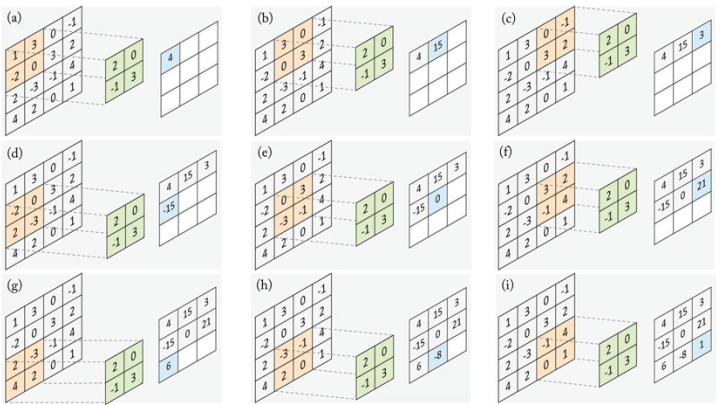
\includegraphics[width=1\textwidth]{filtro_de_red_convolucional}
	\caption[Ejemplo aplicación de un filtro.]{Ejemplo aplicación de un filtro \cite{cnn}.}
	\label{fig:filtro}
\end{figure}

Los pesos del filtro permanecen fijos a lo largo de la misma ejecución del algoritmo anterior aunque durante el entrenamiento se van ajustando a través de un proceso de retropropagación y descenso de gradiente.

Hay tres hiperparámetros que afectan al volumen de salida:

\begin{itemize}
	\item{Número de filtros}: afecta a la profundida de la salida, ya que cada filtro produce su mapa de características.
	
	\item{Stride}: es la distancia,  o el número de píxeles, que el kernel mueve sobre la matriz de entrada.
	
	\item{zero-padding}: Se utiliza para ajustar los filtros al tamaño de la imagen de entrada.
	pone a 0 todos los elemnetos que quedan fuera de la matriz de entrada. Hay tres tipos:
	
	\subitem{Valid padding}: O no padding, en este caso la última convolución se descarta si las dimensiones no se alinean.
	
	\subitem{Same padding}: Este garantiza que la capa de salida tenga el mismo tamaño que la de entrada. Es el utilizado en este trabajo.
	
	\subitem{Full padding}: Este aumenta el tamaño de la capa de salida añadiendo ceros en el borde de la entrada.
	
\end{itemize}

Después de cada convolución la red aplica una transformación de unidad lineal rectificada (ReLU) al mapa de características introduciendo no linealidad en el modelo. Esto eliminará los números negativos de este.
Después de una primera capa convolucional puede ir otra como ya se ha comentado.

\subsubsection{Capa de agrupación}
La agrupación de capas o submuestreo, permite reducir la dimensión mediante la reducción de los parámetros de la entrada. Este aplica una función de agregación a los valores dentro del campo receptivo y llena la matriz de salida.

Hay dos tipos de agrupación:
\begin{itemize}
	\item{Agrupación máxima}: a medida que recorre la entrada manda el pixel con el valor mayor a la matriz de salida.
	\item{Agrupación media}: a medida que recorre la entrada manda el valor medio de los pixeles dentro del campo receptivo a la matriz de salida
\end{itemize}

Aunque se pierde mucha información en la capa de agrupación esto ayuda a reducir la complejidad, mejora la eficiencia y limita el riesgo de sobreajuste. 

\subsubsection{Capa totalmente conectada}
Esta capa realiza la predicción en base a los mapas de características de las capas anteriores contra la imágen original. Suele usar una función softmax que clasifica valores de entre 0 y 1. En el caso de este experimento se utiliza una funcion sigmoid al ser una clasificación binaria.

\subsection{Red convolucional U-Net}
En este apartado explicaremos el funcionamiento de la red U-Net, un tipo de red convolucional muy utilizado para análisis de imágenes, el cual ha sido implementado en este experimento. Este es una mejora a otras redes convolucionales aumentando la precisión y pudiendo hacer clasificaciones más ajustadas.

Para comprender correctamente la arquitectura de la red U-Net \cite{Unet} es recomendable ver la figura~\ref{fig:red_U-Net}.

La red U-Net es una red neuronal convolucional qeu se divide en dos partes, el camino de expansión y el camino de compresión. La red empieza aplicando dos capas convolucionales a la imágen, separando en 64 mapas de características las imágenes y pasando a la siguiente capa estas además de pasandolo a la capa reflejada en el camino de expansión. La siguiente capa es una capa de agrupación, la cual se encarga de reducir su dimensionalidad. este proceso se repite en todo el camino de contracción. Una vez acaba el proceso de contracción se hace el proceso inverso para el proceso de expansión, sumando los mapas de características que se han obtenido en el camino de contracción.

\begin{figure}[H]
	\centering
	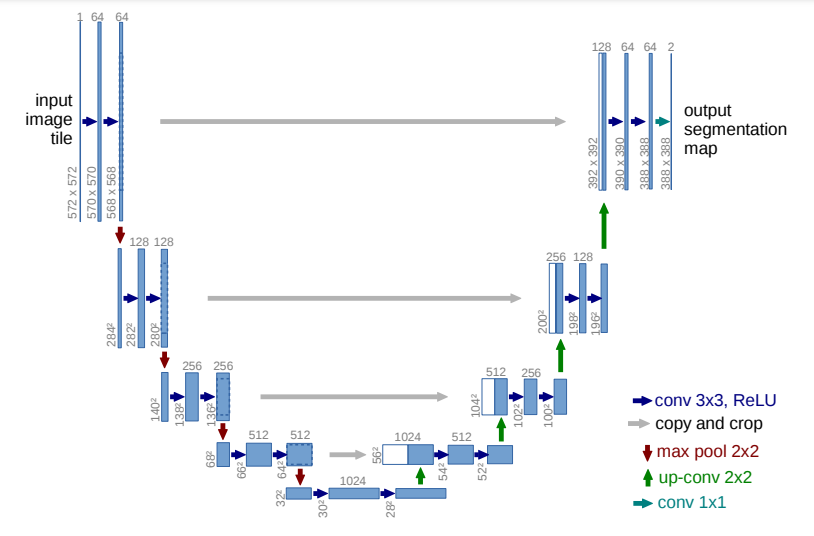
\includegraphics[width=1\textwidth]{red_U-Net}
	\caption[Funcionamiento red U-net.]{Funcionamiento red U-net \cite{Unet}.}
	\label{fig:red_U-Net}
\end{figure}

\chapter{Técnicas y herramientas}

En este apartado se explicarán el grueso de las herramientas utilizadas para este proyecto.

\section{Python}
El lenguaje de programación que se ha utilizado en este proyecto ha sido Python. Este es un lenguaje de programación creado por Guido van Rossum a principios de los años 90 cuyo nombre está inspirado en el grupo de cómicos ingleses “Monty Python”\cite{gonzalez2011python}. Su sintexis se centra en la legibilidad y la limpieza de código.

El lenguaje tiene las siguientes características:
\begin{itemize}
	\item\textbf{Lenguaje interpretado}: Esto significa que para su ejecución requiere otro programa llamado interprete, en lugar de compilar el código a lenguaje máquina y ejecturalo directamente.
	Esto lo convierte en más flexible y portable. Aunque este tiene muchas de las características de los lenguajes compilados.
	
	\item\textbf{Tipado dinámico}: Esto se refiere a que no es necesario declarar los tipos de las variables de manera explícita. Estos tipo se determinarán en tiempo de ejecución. El tipo de las variables puede cambiar con nuevas asignaciones.
	
	\item\textbf{fuertemente tipado}: Esto significa que  no se puede tratar a una variable como si tuviera un tipo distinto del que tiene, han de hacerse las transformaciones de forma explícita.
	
	\item\textbf{multiplataforma}: Este es capaz de correrse en una gran cantidad de sistemas sin cambios significativos.
	
	\item\textbf{Orientado a objetos}: La orientación a objetos es un paradigma de programación en el cual se abstraen los conceptos del mundo real como clases y objetos. Aunque python permite también la programación imperativa y la orientada a aspectos.
	
\end{itemize}

Python no es adecuado para la programación de bajo nivel o para aplicaciones en las que el rendimiento sea crítico.

El principal motivo para la selección de este lenguaje es las librerías que hay desarrolladas para el, como Scikit-learn~\ref{sect:scikit}, NumPy~\ref{sect:numpy} o matplotlib~\ref{sect:matplotlib}.

\section{Jupyter Notebook}

Jupyter Notebook\cite{ionosJupyterNotebook} es una aplicación cliente-servidor que permite crear, compartir y visualizar archivos en formato JSON que siguen un esquema de celdas de entrada y salida.

Las celdas contienen textos, código, fórmulas matemáticas e incluso contenido multimedia. Los archivos se guqardan en formato .ipynb.

Estos permite compartir códigos, ejecutarlos de manera sencilla, proporcionar una interfaz cómoda para albergar las visualizaciones además de intercalar textos explicativos con el código.

Jupyter Notebooks tiene un conjunto de núcleos y el Dashboard. Cada núcleo o kernel es el que se encarga de recibir las peticiones, procesar las solicitudes y devolver las respuestas. El kernel por defecto es IPyhton, el cual interpreta comandos de Python, pero se pueden instalar otros tipos de núcleos que permitan trabajar con otros lenguajes como C++, R, Java o Scala entre otros.

Es de uso gratuito.

\section{matplotlib}\label{sect:matplotlib}

Matplotlib\cite{datascientestMatplotlibTodo} es una librería open source de Python que permite visualizaciones de datos. La visualización de datos es una parte clave del análisis de datos, en este proyecto concreto se utiliza para la visualización de las imágenes tanto obtenidas de los datos como generadas por el programa.

Se creó en 2002 por Jhon Hunter como una alternativa a MATLAB para visualizar gráficas. La comunidad lo ha mejorado a lo largo del tiempo. 

Permite generar trazados, histogramas y gráficas de gran calidad. 

\section{NumPy}\label{sect:numpy}

NumPy\cite{bressert2012scipy} es un paquete de Python que incluye operaciones complejas como operaciones con vectores de N dimensiones, matrices, integrales, ecuaciones diferenciales , estadísticas y más. Python tiene implementadas por defecto algunas funciones matemáticas pero no adecuadas para matrices y vectores. NumPy permite el uso eficiente de Python para propósitos científicos.

NumPy se especializa en el procesado de vectores multidimensionales, en los que se permiten operaciones elemento a elemento. Se puede usar álgebra lineal si es necesario sin modificar previamente los vectores. Se pueden redimensionar las matrices de manera dinámica. Esto es más rápido y eficiente que en otros lenguajes ya que evita el tener que crear nuevos vectores. 

Los vectores de NumPy permiten incrustar código en C/C++/Fortran, lo que aumenta sobremanera su eficiencia.Una operación con ndarray es 25 más rápido que un bucle de python. Los ndarrays solo pueden almacenar un tipo de dato por columna. 
 
\section{Scikit-learn}\label{sect:scikit}

Scikit-learn es un modulo de Python que integra un amplio rango de algoritmos para problemas de aprendizaje tanto supervisado como no supervisado. Este se enfoca como un paquete que acerca las técnicas de \textit{machine learning} a personas no especializadas en el campo, de forma general en un lenguaje de alto nivel.  Usa una interfaz orientada a las tareas.

Tiene dependencias externas mínimas y se distribuye  con una licencia de BDS simplificada, es decir como un software libre.

También incorpora código compilado y librerías en C++ para aumentar la eficiencia. Para reducir las barreras de entrada reducen al mínimo los objetos propios y trata de utilizar los objetos de NumPy para almacenar datos.

Proporciona una documentación muy completa con tutoriales varios.

\section{TensorFlow y Keras}

TensorFlow\cite{TensorYKeras}\cite{TensorYKeras2} es uno de los frameworks de inteligencia artificial más conocidos y utilizados. fue desarrollado originalmente por el grupo de Google Brain. Fue diseñado para facilitar la investigación en \textit{machine learning} y realizar más rápida la transición de un prototipo a un sistema de producción. 

Keras es una API de alto nivel para redes neuronales. El código se especifica en Pyhton y es capaz de ejecutarse en tres entornos : TensorFlow, CNTK o Theano. Se puede cambiar de motor de ejecución sin alterar el código. TensorFlow ha decidido adoptar Keras como su API principal. Los modelos de Keras se pueden crear mediante APIs secuenciales de 'tf.keras.Sequential' o mediante la API funcional de Keras 'tf.keras.Model'.

TensorFlow proporciona un grupo de paquetes relacionados con la creación de redes neuronales. Estos facilitan la creación y personalización de las capas (tf.keras.layers), datasets (tf.data), métricas (tf.keras.metrics), funciones de perdida (tf.keras.losses) y columnas de características (tf.feature\_column).



\chapter{Aspectos relevantes del desarrollo}
En este apartado se explicarán los experimetos realizados y las conclusiones obtenidas a lo largo de estos.

\section{Obtención de los datos de prueba}\label{sect:datosPrueba}
Como se ha comentado previamente los datos se obtienen del proyecto \textit{``AI4Boundaries: an open AI-ready dataset to map field boundaries with Sentinel-2 and aerial photography''} \cite{AI4boundaries}, concretamente del  \href{https://jeodpp.jrc.ec.europa.eu/ftp/jrc-opendata/DRLL/AI4BOUNDARIES/}{repositorio de datos} del proyecto.

Como podemos ver se organizan en varias 3 carpetas:

\begin{itemize}
	\item{Orthophotos}: Carpeta dónde aparecen las Ortofotos del proyecto. Estas no son utilizadas en este proyecto.
	\item{Sampling}: Carpeta dónde se almacenan los csv que relacionan las distintas imágenes con su respectiva url en el ftp sobre el repositorio, tanto la imagen en formato .nc como las máscaras de capa .tif. Esta carpeta tampoco se ha utilizado ya que las imágenes se han descargado para las pruebas en lugar de hacer una carga dinámica.
	\item{Sentinel2}: Carpeta que guarda tanto las imágenes como las máscaras además de archivos csv que muestran cuantos píxeles de cada tipo tienen los resultados.
\end{itemize}

Por la cantidad de datos y los recursos de los que dispone el sistema se ha decidido trabajar solo con un subconjunto de los datos, concretamente los correspondientes a 128 imágenes de España.

\section{Visualización de los datos y composición de la imagen}
Lo primero que se realizó fue una exploración de los datos, para comprender mejor estos y ver sus estructuras, para eso se extrajeron las bandas 4, 3 y 2, correspondientes a la banda Roja, Verde y Azul, se visualizaron en como podemos ver en la figura ~\ref{fig:bandas_rgb} y posteriormente se compusieron en una imágen RGB como podemos ver en la figura ~\ref{fig:imagen_compuesta}.

\begin{figure}[H]
	\centering
	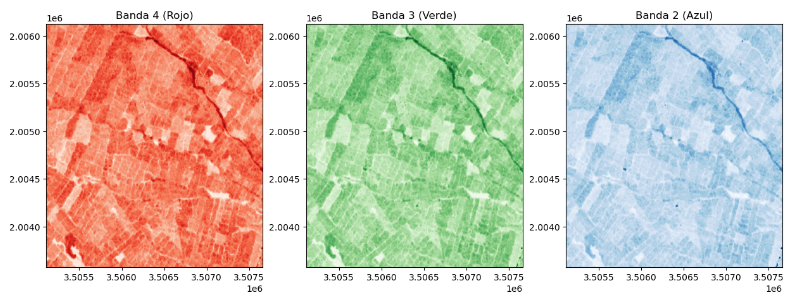
\includegraphics[width=1\textwidth]{Bandas_RGB_separadas}
	\caption[Visualización de las Bandas RGB separadas]{Visualización de las Bandas RGB separadas.}
	\label{fig:bandas_rgb}
\end{figure}

\begin{figure}[H]
	\centering
	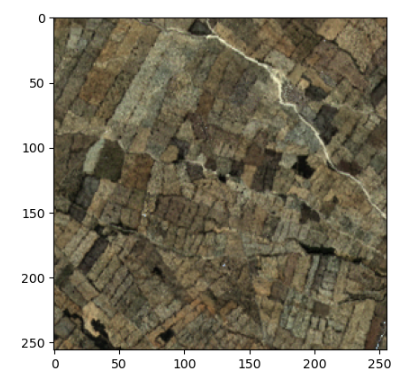
\includegraphics[width=0.4\textwidth]{Imagen_compuesta}
	\caption[Visualización de la imagen compuesta con las bandas RGB]{Visualización de la imagen compuesta con las bandas RGB.}
	\label{fig:imagen_compuesta}
\end{figure}

Una vez visualizada la imagen se comprobó cómo son las máscaras de capa, estas tienen 4 capas distintas la máscara de capa, una mascara de límites,una mascara de distancia y una enumeración de campos. Se ha decidido entrenar los modelos con la primera opción. Como podemos ver en la figura ~\ref{fig:mascara_sola}.

\begin{figure}[H]
	\centering
	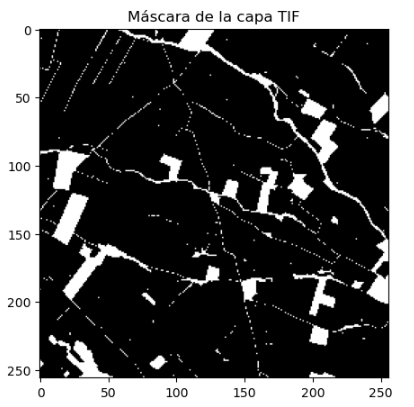
\includegraphics[width=0.66\textwidth]{Mascara_tif}
	\caption[Visualización de la máscara de capa de las delimitaciones]{Visualización de la máscara de capa de las delimitaciones.}
	\label{fig:mascara_sola}
\end{figure}

Tras eso se superpuso la capa con la imagen para comprobar cuánto se adecua con la imagen. Como se puede ver en la figura  ~\ref{fig:mascara_superpuesta} registran los grandes límites.

\begin{figure}
	\centering
	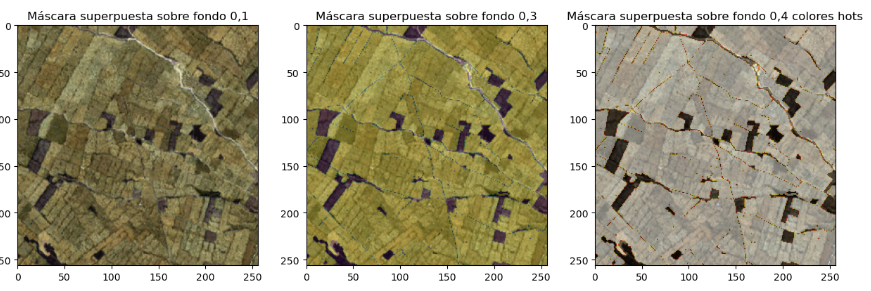
\includegraphics[width=1\textwidth]{Mascara_superpuesta}
	\caption[Visualización de la máscara de capa superpuesta con la imagen]{Visualización de la máscara de capa superpuesta con la imagen.}
	\label{fig:mascara_superpuesta}
\end{figure}

 
\section{Modelos sin contexto}
En este apartado intentaremos entrenar tres modelos: KNN, SVM y RandomForest. Estos no tienen en cuenta el contexto de los píxeles, predicen unicamente en base a la información de cada píxel por lo que se asumía, cosa que se comprobó que obtienen unos resultados peores. 

\subsection{KNN}
Se empezó por KNN, este tuvo un tiempo de entrenamiento de 57.88 segundos. Se hizo una predicción sobre la imagen del inicio para poder visualizar el resultado. Los resultados son la figura ~\ref{fig:prediccion_knn}.

\begin{figure}[H]
	\centering
	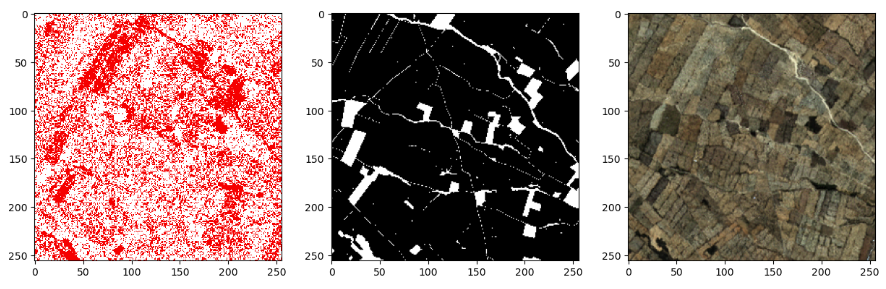
\includegraphics[width=1\textwidth]{Clasificacion_KNN}
	\caption[Visualización de la predicción sobre la imagen KNN]{Visualización de la predicción sobre la imagen por el modelo KNN comparada con el resultado previsto y la imagen orginal.}
	\label{fig:prediccion_knn}
\end{figure}

\begin{figure}[H]
	\centering
	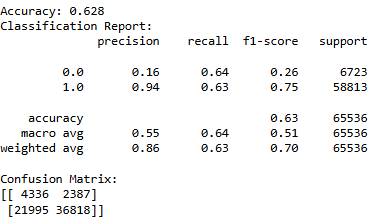
\includegraphics[width=0.66\textwidth]{Metricas_KNN}
	\caption[Métricas obtenidas para el modelo KNN]{Métricas obtenidas para el modelo KNN.}
	\label{fig:metricas_knn}
\end{figure}

Las métricas obtenidas por el modelo han sido las mostradas en la figura ~\ref{fig:metricas_knn}. 
Si se analizan los resultados podemos ver que si bien reconoce algunas estructuras y se puede llegar a intuir la imagen en la predicción, hay mucho ruido en la imagen y probablemente el hecho de que haya obtenido unos resultados es derivado de que es un conjunto de datos relativamente desbalanceado.

\subsection{SVM}
El siguiente modelo a probar es SVM, el cual no se pudo llegar a entrenar ya que el tiempo que requirió  para entrenarse era claramente excesivo superando las 16 horas antes de que se decidiera pararlo.

\subsection{Random Forest}
Finalmente Se probó Random Forest, el cual se lanzo con todos los núcleos posibles en paralelo, de cara a mejorar su eficiencia. igualmente tuvo un tiempo de entrenamiento de 1273.35 segundos. Se pueden ver los resultados de la predicción en la figura ~\ref{fig:prediccion_rf} y las métricas ~\ref{fig:metricas_rf}.


\begin{figure}[H]
	\centering
	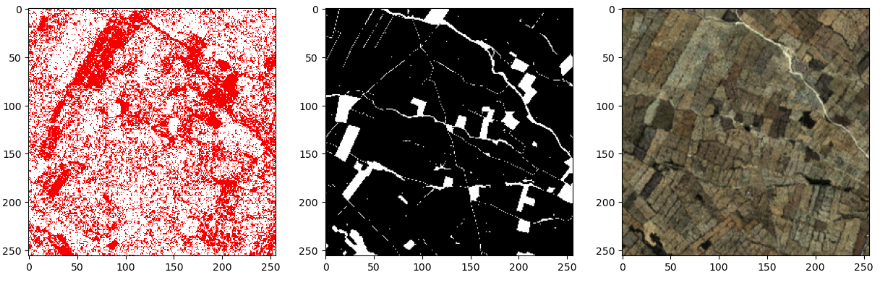
\includegraphics[width=1\textwidth]{Clasificacion_Random_Forest}
	\caption[Visualización de la predicción sobre la imagen Random Forest]{Visualización de la predicción sobre la imagen por el modelo Random Forest comparada con el resultado previsto y la imagen orginal.}
	\label{fig:prediccion_rf}
\end{figure}

\begin{figure}[H]
	\centering
	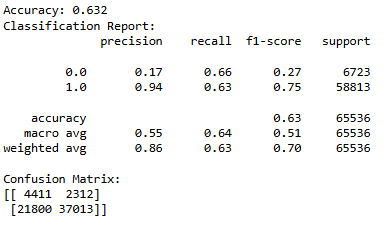
\includegraphics[width=0.66\textwidth]{Metricas_Random_Forest}
	\caption[Métricas obtenidas para el modelo Random Forest]{Métricas obtenidas para el modelo Random Forest.}
	\label{fig:metricas_rf}
\end{figure}

\section{Modelo U-Net}
Finalmente el grueso de las pruebas se hicieron son las relacionadas con la red convolucional de tipo U-Net. Esta como ya se ha mentado tiene contexto de los píxeles alrededor del que se está analizando. Esto de manera teórica se supone que obtendrá mejores resultados, cosa que se ha probado.

Se empezó por implementar la red neuronal, siguiendo los pasos del paper \cite{Unet} aunque se implementó una segunda versión en la cual hay Dropout en tre las convoluciones de una misma capa, para evitar el sobreajuste.

En todas las opciones se escogió como optimizador adam, como métricas accuracy y como función de perdida binary\_crossentropy. Estos han tenido un tiempo de entrenamiento por época de entre 250 y 300 segundos. Marcando un accuracy según las métricas de Keras de entre 0.75 y 0.86 siendo a partir de 10 épocas normalmente superiores a 0.8.

De cara a buscar cual es la mejor configuración posible se probaron en un inicio 8 modelos, los cuales se hizo una predicción sobre la imagen previa para visualmente analizar cual ha sido más adecuado. Se muestra en la figura ~\ref{fig:predicciones}.

\begin{figure}
	\centering
	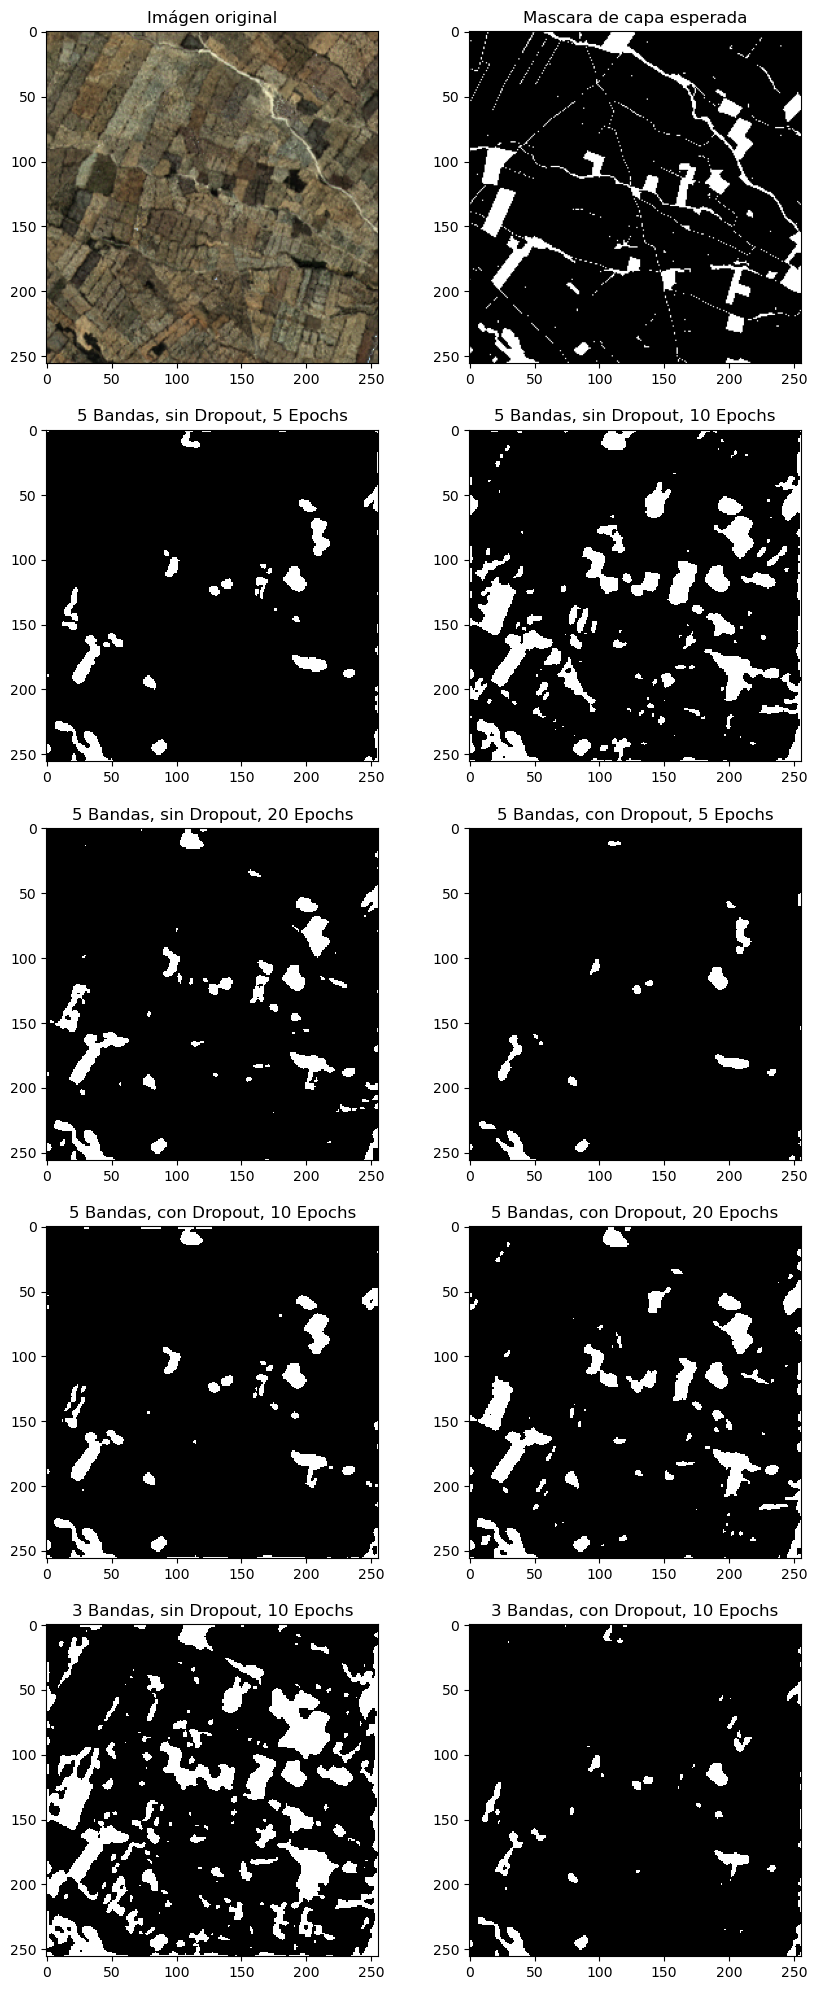
\includegraphics[scale=0.4]{resultados_unet}
	\caption[Predicciones realizadas por los modelos descritos]{Predicciones realizadas por los modelos descritos.}
	\label{fig:predicciones}
\end{figure}

Finalmente viendo los resultados dados se decidió entrena un modelo más esta vez con 40 épocas y con dropout, que será el modelo a utilizar.
Los resultados de este lo podemos ver en la figura ~\ref{fig:prediccion_540c}.
	
\begin{figure}[H]
	\centering
	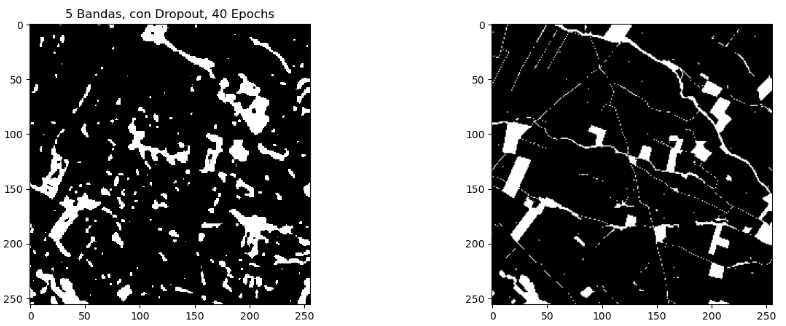
\includegraphics[width=1\textwidth]{Unet_clasificacion_5_bandas_40_epocas_con_dropout}
	\caption[Predicción realizada por el modelo final]{Predicción realizada por el modelo final.}
	\label{fig:prediccion_540c}
\end{figure}

Es reseñable que si bien este muestra esa predicción con un umbral de predicción de 0.5, entendiendo que este es el punto a partir del cual en la predicción se considera 1. La predicción sin hacer ese filtrado por umbral muestra una imagen muy interesante que puede ser más interpretable como se puede ver en la figura ~\ref{fig:prediccion_sin_umbral}.
	
\begin{figure}[H]
	\centering
	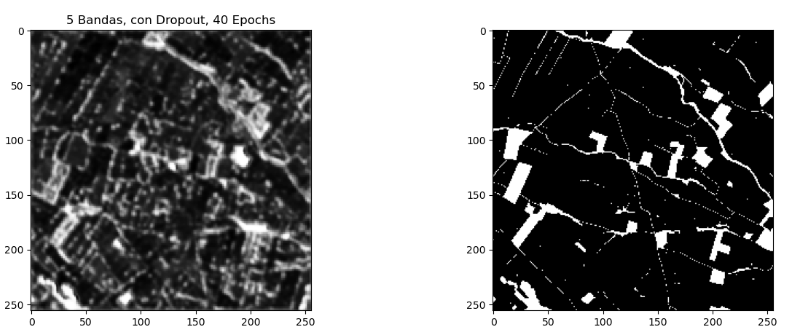
\includegraphics[width=1\textwidth]{Unet_clasificacion_5_bandas_40_epocas_con_dropout_sin_threshold}
	\caption[Predicción realizada por el modelo final sin binarizar]{Predicción realizada por el modelo final sin binarizar.}
	\label{fig:prediccion_sin_umbral}
\end{figure}

Finalmente se evaluaron los modelos y el que mejores métricas consiguió fue el último, tal y como se había predicho. Este tienes las métricas mostradas en la siguiente figura  ~\ref{fig:metricas_u-net}.

\begin{figure}[H]
	\centering
	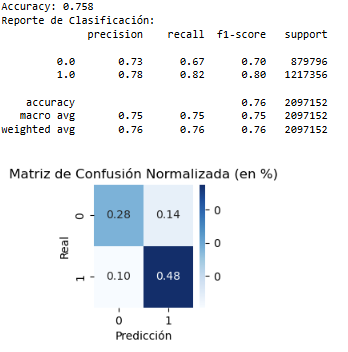
\includegraphics[width=1\textwidth]{metricas_u-net}
	\caption[Métricas del modelo U-Net con 40 Epochs]{Métricas del modelo U-Net con 40 Epochs con dropout.}
	\label{fig:metricas_u-net}
\end{figure}

Analizando estos resultados se puede reseñar que se han obtenido un modelo suficientemente adecuado, aunque puede llegar a ser mejorable.
\chapter{Trabajos relacionados}
En este apartado se comentarán algunos de los trabajos relacionados y experimentos similares.

\section{AI4Boundaries: an open AI-ready dataset to map field boundaries with Sentinel-2 and aerial photograph \cite{AI4boundaries}}

Este es el artículo sobre el que se basa este trabajo, ya que es el que proporciona los materiales para el entrenamiento de los modelos sin los cuales esta tarea hubiera muchísimo más ardua y probablemente de una calidad muy inferior.

El artículo presenta AI4Boundaries, un conjunto de datos abierto y preparado para el aprendizaje automático que tiene como objetivo facilitar la detección de límites de campos agrícolas utilizando imágenes de satélite Sentinel-2 y fotografías aéreas.
\begin{itemize}

	\item El conjunto de datos incluye dos componentes principales:
	Una composición mensual de imágenes Sentinel-2 a una resolución de 10 metros, lo que permite el análisis a gran escala.
	
	\item Ortofotografías aéreas a una resolución de 1 metro, lo que posibilita el análisis a escala regional.
\end{itemize}

Los datos de etiquetado de los límites de campos provienen de fuentes públicas, como el Sistema Integrado de Gestión y Control (SIGC) de varios países europeos, como Austria, Cataluña, Francia, Luxemburgo, Países Bajos, Eslovenia y Suecia.

El conjunto de datos ha sido diseñado para ser utilizado en el entrenamiento de modelos de aprendizaje automático que puedan realizar la delineación automática de los límites de campos agrícolas.

\section{U-Net: Convolutional Networks for Biomedical Image Segmentation \cite{Unet}}

Este es el artículo que da la arquitectura del modelo principal de este trabajo, la red convolucional de tipo U-Net. Esta está diseñada para la segmentación de imágenes biomédicas. Se basa en la red convolucional completamente conectada (FCN) y se modifica para funcionar con pocos datos de entrenamiento y producir segmentaciones más precisas.

Este artículo trata de resolver el problema de que el entrenamiento de redes profundas requiere generalmente miles de muestras de entrenamiento etiquetadas. Sin embargo, en tareas biomédicas, como la segmentación de imágenes, es difícil obtener tantos datos etiquetados.

Esto lo soluciona a través de las de dos fases:

\begin{itemize}
	
	\item{Contracción}: Un camino de contracción que captura el contexto mediante la aplicación repetida de convoluciones 3x3, seguidas de ReLU introduciendo no linealidad al modelo y operaciones de pooling máximo de 2x2 con un salto de 2 para la reducción de la información espacial y el aumento de la información de características. A medida que el modelo pasa por estas fases le pasa el mapa de características resultante a la capa correspondiente en la segunda fase, siendo esta la capa de su mismo número de mapas de características.
	
	\item{Expansión}: Un camino de expansión que combina la información de características y espacial a través de la concatenación de características de alta resolución de la ruta de contracción con las características de alta resolución de la ruta de expansión.
	En esta fase se aplican las mismas que en la anterior pero en orden inverso.
	
\end{itemize}

La U-Net representa una herramienta valiosa para la comunidad científica y los profesionales del sector biomédico, al proporcionar una arquitectura de red que puede ser entrenada de manera eficiente con pocos datos y producir segmentaciones precisas y rápidas.

Este método superó a los métodos anteriores tanto en velocidad como en precisión.

\chapter{Conclusiones y lineas de trabajo futuras}
En este apartado se hará una rendición de cuentas respecto a los objetivos marcados, se explicarán las conclusiones que se han extraído y finalmente se comentarán posibles líneas de trabajo futuras.

\section{Conclusiones}
Las conclusiones que podemos obtener de este proyecto son las siguientes:

\begin{itemize}
	\item Las redes neuronales convolucionales son una herramienta muy útil para la clasificación de imágenes. Si bien hay otros modelos capcaes de realizar la tarea de manera apróximada este es el mejor de los probados.
	
	\item Existen técnicas automáticas para la separación automática de parcelas capaces de realizar la tarea satisfactoriamente.

\end{itemize}

\section{Rendición de cuentas}
Se expondrán en esta sección los objetivos marcados en el episodio previo y se comentará el estado de los mismos.

\begin{itemize}
	\item Entrenar un modelo capaz de realizar una separación suficiente de parcelas en base a una imagen satelital. 
	
	Se da por cumplido este objetivo, si bien es relativo que se entiende por suficiente, se consideran suficientemente buenos los resultados obtenidos.
	
	\item Probar diferentes métodos y configuraciones de cara a comprobar si realmente la red neuronal convolucional es el método más potente o pueden ser más interesantes otras metodologías que impliquen que no tener en cuenta el contexto de los píxeles.
	
	Con respecto a este apartado se puede considerar como comprobado, analizando las métricas de los modelos explorados podemos ver que las mejores métricas obtenidas han sido las de los modelos predichos. Además se han probado diversos modelos, si bien es cierto que SVM no ha sido posible el tiempo de entrenamiento excesivo ya lo hubiera descartado como viable.
	
	\item Exponer los conocimientos extraídos en un notebook de Python, lo cuál facilitará la trasmisión y la manipulación de estos.
	
	El Notebook ha sido realizado con éxito.
	
	\item Generar un repositorio dónde almacenar dicho notebook con la estructura definida para una poder ejecutar de forma simple el cuaderno.
	
	El repositorio ha sido creado, en el apartado 5\ref{sect:datosPrueba} se explica como han de almacenarse los archivos y la URL del repositorio es: 
	\href{https://github.com/wgm1001/Trabajo_fin_master_deteccion_bordes}{Repositorio} 
	
	\item Tratar de optimizar en la medida de lo posible los parámetros del modelo para maximizar su eficiencia.
	
	Si bien es cierto que pudieran obtenerse mejores resultados, se consideran suficientes las pruebas realizadas, ahora en este punto es en el que más se puede mejorar, cosa de la que hablaremos en el apartado de Líneas de trabajo futuras\ref{sect:lineasFuturas}.
		
\end{itemize}

\section{Líneas de trabajo futuras}\label{sect:lineasFuturas}
Respecto a las posibles mejoras y líneas de trabajo futuras:
\begin{itemize}
	\item Probar a entrenar el modelo con un número mayor de imágenes y una mayor variedad.
	
	Si bien es cierto que los resultados son suficientes con el número de imágenes reducido que se han utilizado, es posible que al usar una mayor parte del Dataset los resultados puedan ser mejores.
	
	\item Probar más parámetros.
	
	Dentro de los parámetros que se pueden manipular para cambiar los resultados en este trabajo sobre todo se han probado las épocas, el número de bandas y la posibilidad de hacer dropout o no, pero como hemos visto en el apartado 3\ref*{sect:redesConvolucionales} hay muchos hiperparámetros que se pueden modificar además de alguno más derivado de la definición del modelo o incluso el umbral de corte.

	\item Hacer un programa que sea capaz de analizar imágenes.
	
	Puede ser interesante hacer un programa que sea capaz de dada una imagen satélite haga la separación. También se podrían automatizar las descargas de los documentos del ftp para no requerir de almacenarlos en memoria.
		
\end{itemize}


\renewcommand\chaptername{Anexo}
\renewcommand\thechapter{\Roman{chapter}}
\setcounter{chapter}{0}

% Añadir entrada en el índice: Anexos
\appendix
\addcontentsline{toc}{part}{Apéndices}
\part*{Apéndices}

\include{./tex/A_Plan_de_proyecto}
%\include{./tex/B_Requisitos}
%\include{./tex/C_Diseno}
\apendice{Manual de programador}
En este manual se indicarán los pasos a seguir para la ejecución del Notebook.

Lo primero que se ha de hacer tener instalado o instalar Python, preferentemente en su versión 3.11.5 que es en la que se ha desarrollado, aunque seguramente no den problemas versiones más nuevas.

También han de instalarse las siguientes dependencias:
\begin{itemize}
	\item Numpy
	\item Matplotlib
	\item Seaborn
	\item Scikit-learn
	\item Tensorflow
\end{itemize}
Todas ellas se pueden instalar mediante pip install, incluso si se quiere desde el propio notebook.

Tras lo cual será necesario instalar Jupyter Notebook. La forma sencilla sería hacer, la guía propia de Jupyter se encuentra en el siguiente \href{https://jupyter.org/install}{enlace}:
pip install jupyterlab

Una vez instalado se debe iniciar mediante el comando jupyter notebook, al ejecutarlo se proveerá de un enlace para navegar desde el programa. 

Se ha de clonar el \href{https://github.com/wgm1001/Trabajo_fin_master_deteccion_bordes}{repositorio de del proyecto} ``wgm1001 / Trabajo\_fin\_master\_deteccion\_bordes'' de gitHub o bien descargarlo.

Como se ha comentado previamente los datos se obtienen del proyecto \textit{``AI4Boundaries: an open AI-ready dataset to map field boundaries with Sentinel-2 and aerial photography''} \cite{AI4boundaries}, concretamente del  \href{https://jeodpp.jrc.ec.europa.eu/ftp/jrc-opendata/DRLL/AI4BOUNDARIES/sentinel2/}{repositorio de datos} del proyecto.

Para una ejecución similar a la del proyecto y sin tiempos excesivos se recomienda escoger solo los datos que inician por ES.

Una vez descargados Las imágenes .nc de entrenamiento las almacenamos en la carpeta ``/data/trainES/'', las de test en la carpeta ``/data/test/'' y las máscaras de capa de los resultados \textit{ground truth} en la carpeta ``/data/maskES/'' para las de los datos de entrenamiento y ``/data/maskTestEs/'' para el test.

También el archivo ``ES\_126\_S2\_10m\_256'' tanto .nc como .tif en la carpeta ``data'' ya que es el que se ha utilizado para todas las visualizaciones.

Una vez están todos los archivos en su correspondiente localización, desde el navegaro en la aplicación de Jupyter se ha de navegar hasta en archivo ipynb. Ya se pueden correr de manera secuencial todas las celdas menos la del SVM. La primera vez que se ejecuten se han de entrenar los modelos. en posteriores ejecuciones con ejecutar las celdas en las que se cargan debiera bastar para usarlos. No se pueden subir al repositorio los modelos entrenados  por su tamaños excesivo.
%\include{./tex/E_Manual_usuario}


\bibliographystyle{plain}
\bibliography{bibliografia}

\end{document}
